\documentclass[a4paper,12pt]{report} % добавить leqno в [] для нумерации слева

%%% Работа с русским языком
\usepackage{cmap}					% поиск в PDF
\usepackage{mathtext} 				% русские буквы в формулах
\usepackage[T2A]{fontenc}			% кодировка
\usepackage[utf8]{inputenc}			% кодировка исходного текста
\usepackage[english,russian]{babel}	% локализация и переносы

\usepackage{graphicx}				%вставка изображений(графиков, в частности)
\usepackage{alltt}

%%% Дополнительная работа с математикой
\usepackage{amsmath,amsfonts,amssymb,amsthm,mathtools} % AMS
\usepackage{icomma} % "Умная" запятая: $0,2$ --- число, $0, 2$ --- перечисление

%% Номера формул
\mathtoolsset{showonlyrefs=true} % Показывать номера только у тех формул, на которые есть \eqref{} в тексте.

%% Шрифты
\usepackage{euscript}	 % Шрифт Евклид
\usepackage{mathrsfs} % Красивый матшрифт

%% Свои команды
\DeclareMathOperator{\sgn}{\mathop{sgn}}

%\setlength\parindent{0ex}
%\setlength\parskip{0.3cm}

\renewcommand{\arraystretch}{1.8}

%%% Заголовок
\author{Волков Павел А-14-19}
\title{Отчет по Лабораторной работе №2}
\date{\today}

\begin{document}

\begin{titlepage}
	\newpage

	\begin{center}
	НАЦИОНАЛЬНЫЙ ИССЛЕДОВАТЕЛЬСКИЙ УНИВЕРСИТЕТ\\
		"МОСКОВСКИЙ ЭНЕРГЕТИЧЕСКИЙ ИНСТИТУТ"\\
	\end{center}

	\vspace{8em}	

	\begin{center}
		\Large Кафедра математического и компьютерного моделирования\\ 
	\end{center}

	\vspace{2em}

	\begin{center}
		\textsc{\textbf{ \Large Численные методы \linebreak Отчет по лабораторной работе №2 \linebreak "Решение нелинейных уравнений" \linebreak Вариант 33}}
	\end{center}

	\vspace{6em}



	\newbox{\lbox}
	\savebox{\lbox}{\hbox{Амосова Ольга Алексеевна}}
	\newlength{\maxl}
	\setlength{\maxl}{\wd\lbox}
	\hfill\parbox{11cm}{
		\hspace*{5cm}\hspace*{-5cm}Студент:\hfill\hbox to\maxl{Волков Павел Евгеньевич\hfill}\\
		\hspace*{5cm}\hspace*{-5cm}Преподаватель:\hfill\hbox to\maxl{Амосова Ольга Алексеевна}\\
		\\
		\hspace*{5cm}\hspace*{-5cm}Группа:\hfill\hbox to\maxl{А-14-19}\\
	}


	\vspace{\fill}

	\begin{center}
		Москва \\2021
	\end{center}

\end{titlepage}

\section*{Задача 2.1}
\subsection*{Постановка задачи}
Методом простой итерации найти вещественные корни алгебраического уравнения $P(x) = 0$ с точностью $\varepsilon = 10^{-8}$

\[
	P(x) = x^6 + 0.9x^5 - 0.2x^3 - 1.3x^2 - 0.7x + 0.1
\]

\subsection*{Решение}
Построим графики функций $P(x)$ и $P'(x)$ и найдем отрезки локализации, проверив, что на концах отрезков производная функции сохраняет знак:

\noindent 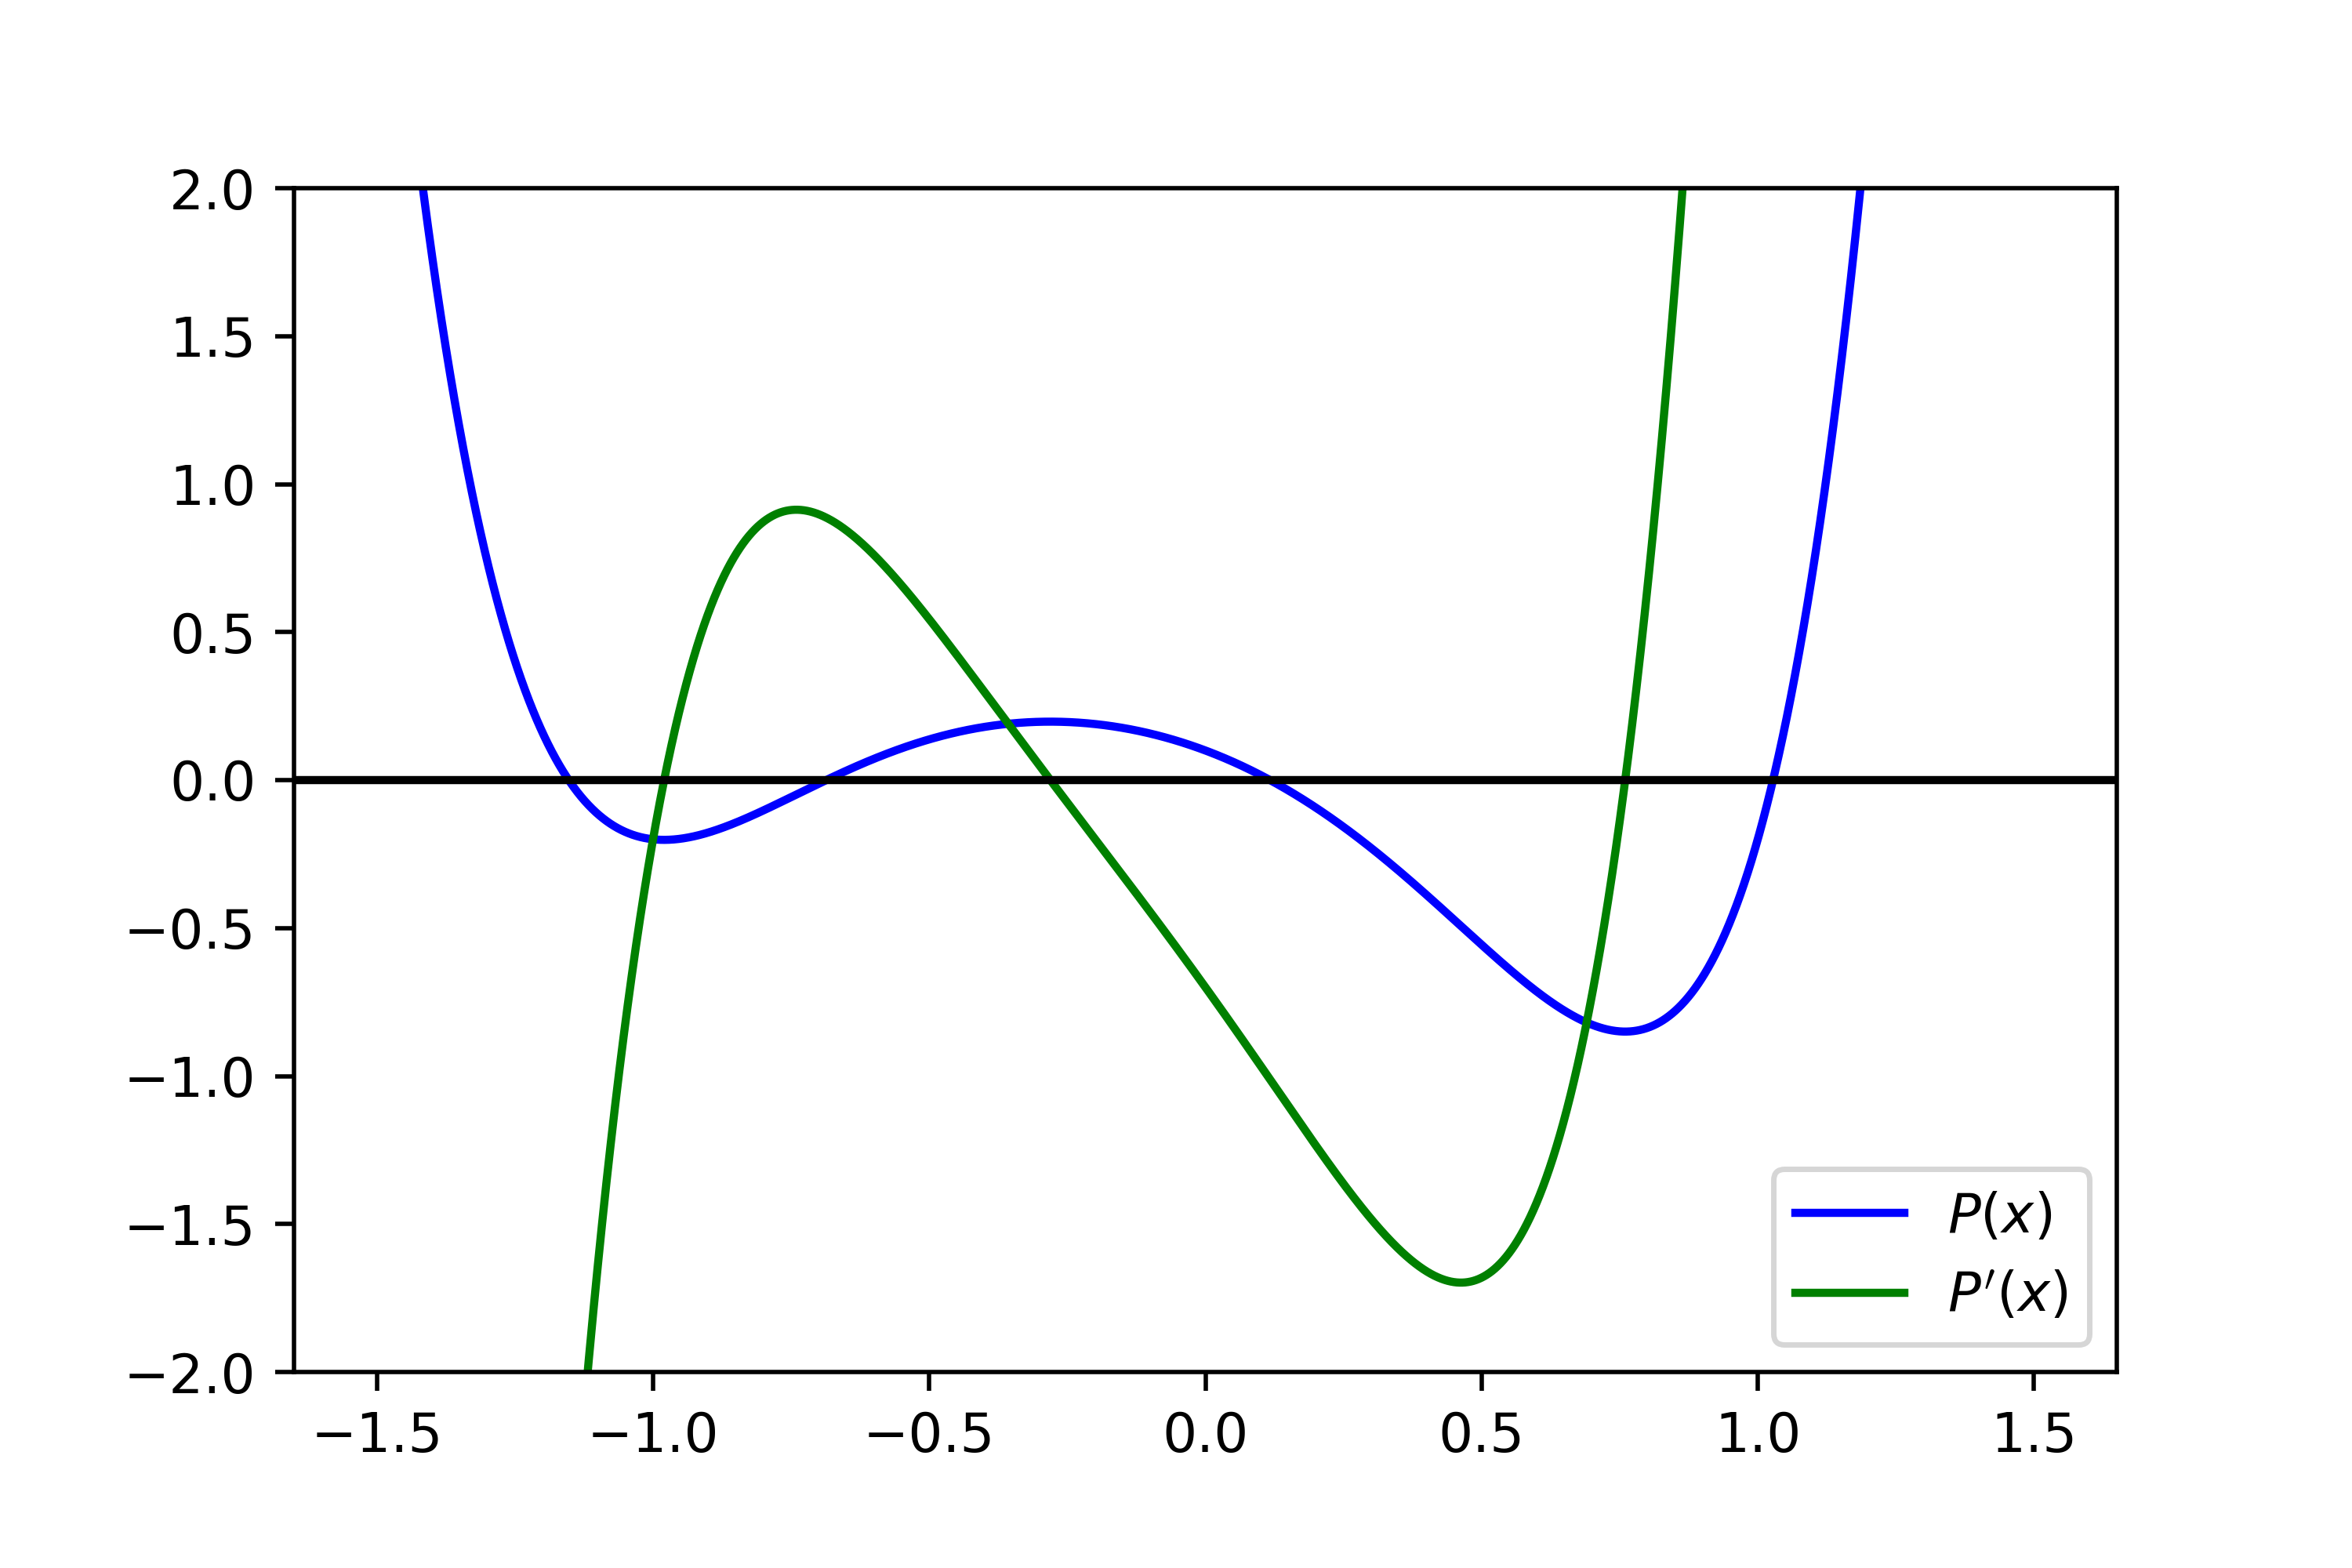
\includegraphics{2.1_plot.png}

Эти четыре корня будут иметь следующие отрезки локализации:
\begin{gather*}
	x_1 \in [-1.4, -1] \\
	x_2 \in [-0.9, -0.5] \\
	x_3 \in [0, 0.5] \\
	x_4 \in [0.8, 1.3]
\end{gather*}

Проверим, что на концах отрезков локализации производная функции сохраняет знак:

\noindent 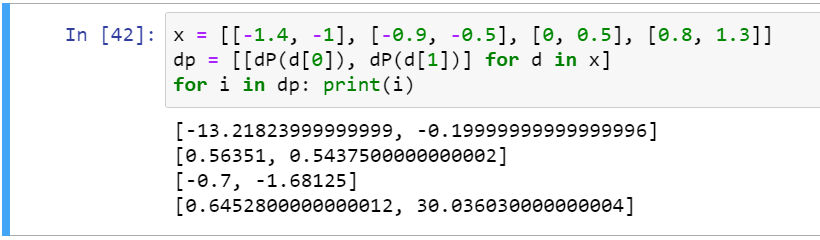
\includegraphics{2.1_dP.png}

Для каждого корня определим итерационный параметр $\alpha$ и $q$:

\begin{gather*}
	M_1 = -0.199, m_1 = -13.218 \\
	M_2 = 0.913, m_2 = 0.544 \\
	M_3 = -0.7, m_3 = -1.698\\
	M_4 = 30.036, m_4 = 0.645 
\end{gather*}

\noindent \begin{tabular}{| c | c | c | c | c |}
	\hline
	Номер корня & 1 & 2  & 3 & 4 \\ \hline
	$\alpha$ & -0.149051  & 1.372510 &  -0.834039 & 0.065186 \\ \hline
	$q$ & 0.970190 & 0.253698 & 0.416173 & 0.957937 \\ \hline
\end{tabular}

\vspace{2em}

Запишем результаты вычислений в таблицу:

\vspace{1em}

\noindent \begin{tabular}{| l | c | c | c | c | c | c |}
	\hline
	\multicolumn{6}{| l |} {ФИО: Волков Павел Евгеньевич, Группа: А-14-19} & Номер варианта: 33 \\ \cline{1-6}
	\multicolumn{6}{| l |} {Уравнение $P(x) = x^6 + 0.9x^5 - 0.2x^3 - 1.3x^2 - 0.7x + 0.1$} & Точность $\epsilon = 10^{-8}$ \\ \hline
	Корни & $[a, b]$ & $M_i$ & $m_i$ & $\alpha$ & $q$ & Число итераций \\ \hline
	1-й: -1.15264767 & $[-1.4, -1]$ & -0.2 & -13.2 & -0.149 & 0.97 & 36 \\ \hline
	2-й: -0.686541063 & $[-0.9, -0.5]$ & 0.913 & 0.544 & 1.37 & 0.254 & 11 \\ \hline
	3-й: 0.117006206 & $[0, 0.5]$ & -0.7 & -1.7 & -0.834 & 0.416 & 9 \\ \hline
	4-й: 1.02764921 & $[0.8, 1.3]$ & 30.0 & 0.645 & 0.0652 & 0.958 & 26 \\ \hline

\end{tabular}

\section*{Задача 2.2}
\subsection*{Постановка задачи}
Дано уравнение $f(x) = 0$. Найти все корни уравнения с заданной точностью $\varepsilon = 10^{-12}$ на указанном отрезке $[a, b]$. Для решения задачи использовать метод Ньютона и метод, указанный в индивидуальном варианте(метод секущих). Сравнить количество итераций, потребовавшихся для достижения заданной точности каждым методом.

\[
	f(x) = \sin{3^x} - \cos{3x} + 0.3, [-1, 2]
\]

\subsection*{Решение}

Построим график функции и локализуем корни уравнения $f(x) = 0$:

\noindent 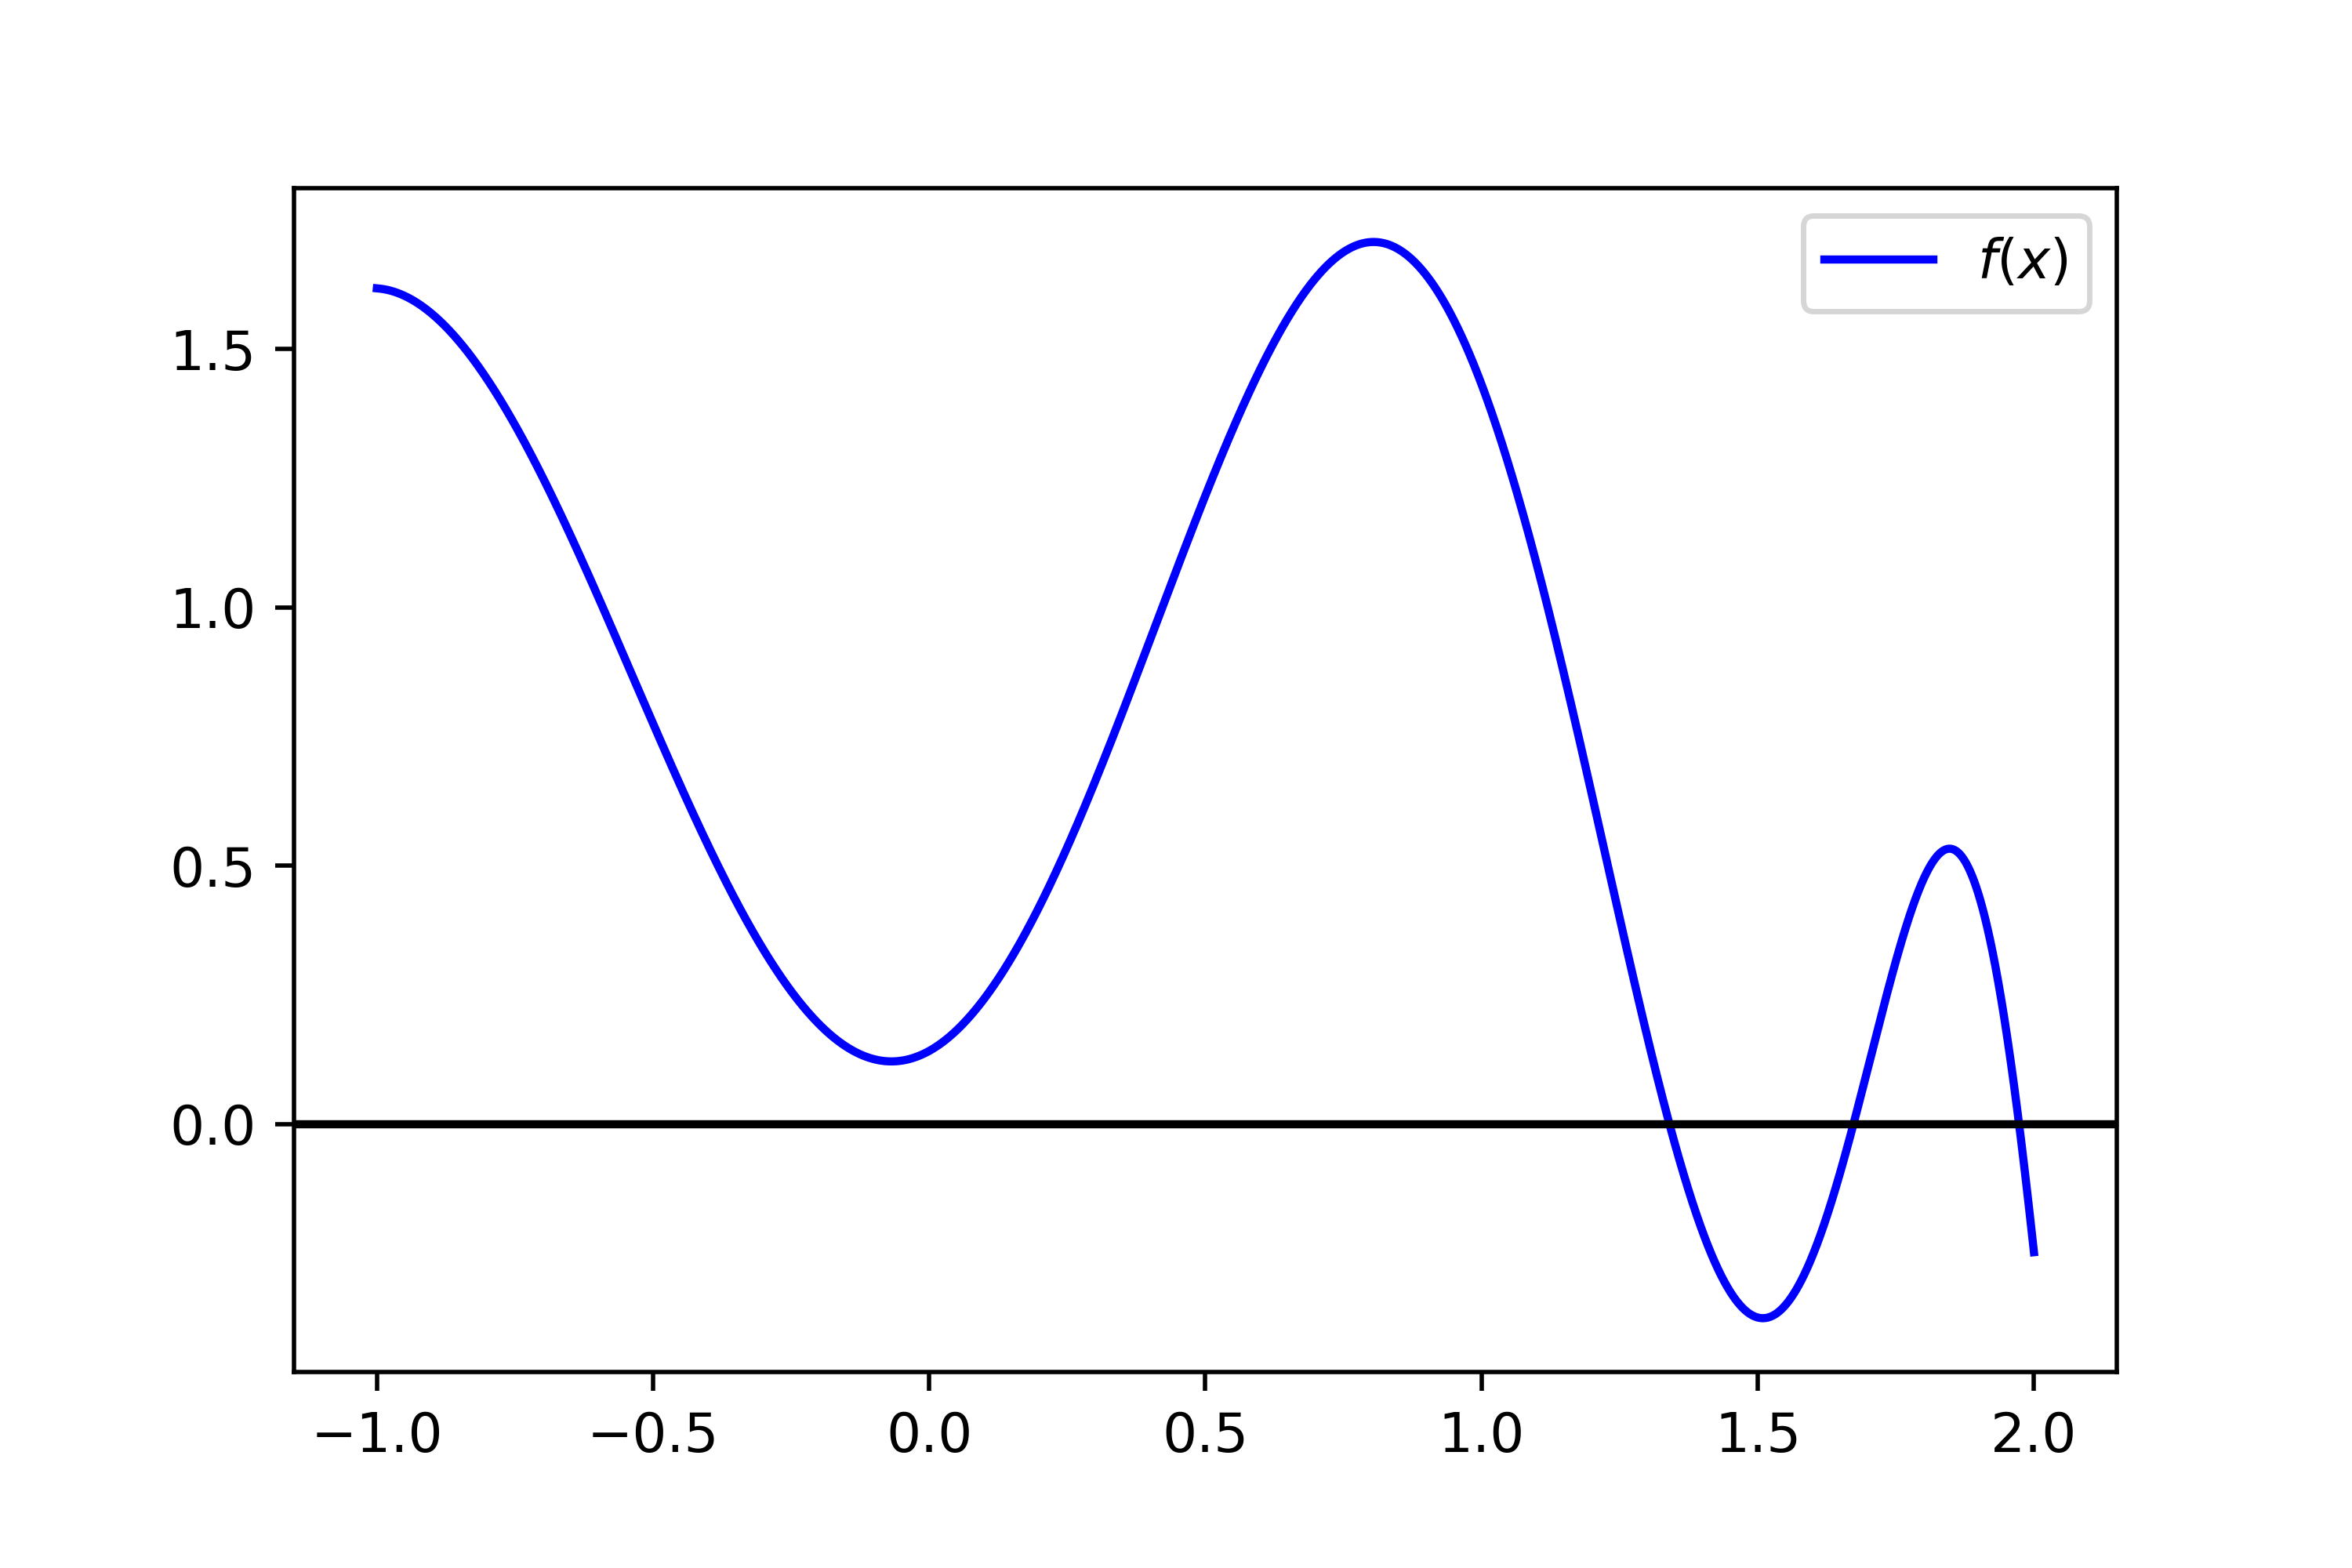
\includegraphics{2.2_plot.png}

Получили 3 корня на следующих отрезках:

\begin{gather*}
	x_1 \in [1.2, 1.4] \\
	x_2 \in [1.6, 1.8] \\
	x_3 \in [1.9, 2]
\end{gather*}

\begin{tabular}{| c | c | c |}
	\hline
	\multicolumn{3}{| l |}{Уравнение: $f(x) = \sin{3^x} - \cos{3x} + 0.3, [-1, 2]$} \\
	\multicolumn{3}{| l |}{Расчетная формула метода Ньютона: $ x^{(k+1)} = x^{(k)} - \frac{f(x^{(k)})}{f'(x^{(k)})}$} \\	
	\multicolumn{3}{| l |}{Расчетная формула метода секущих: $x^{(k+1)} = x^{(k)} - \frac{f(x^{(k)})(x^{(k)} - x^{(k-1)})}{f(x^{(k)}) - f(x^{(k-1)})}$} \\ \hline
	\multicolumn{3}{| c |}{Задача 2.2} \\ \hline
	Корни & Число итераций & Число итераций \\
	уравнения & метода Ньютона & метода секущих \\ \hline
	1.3400823839084 & 6 & 8 \\ \hline
	1.6732949336289 & 5 & 7 \\ \hline
	1.9730518797929 & 6 & 8 \\ \hline
\end{tabular}

\newpage

Модифицируем методы для нахождения модуля невязки $r_n = |f(x_n)|$ на каждой итерации и построим сравнительные графики для каждого из корней:

\noindent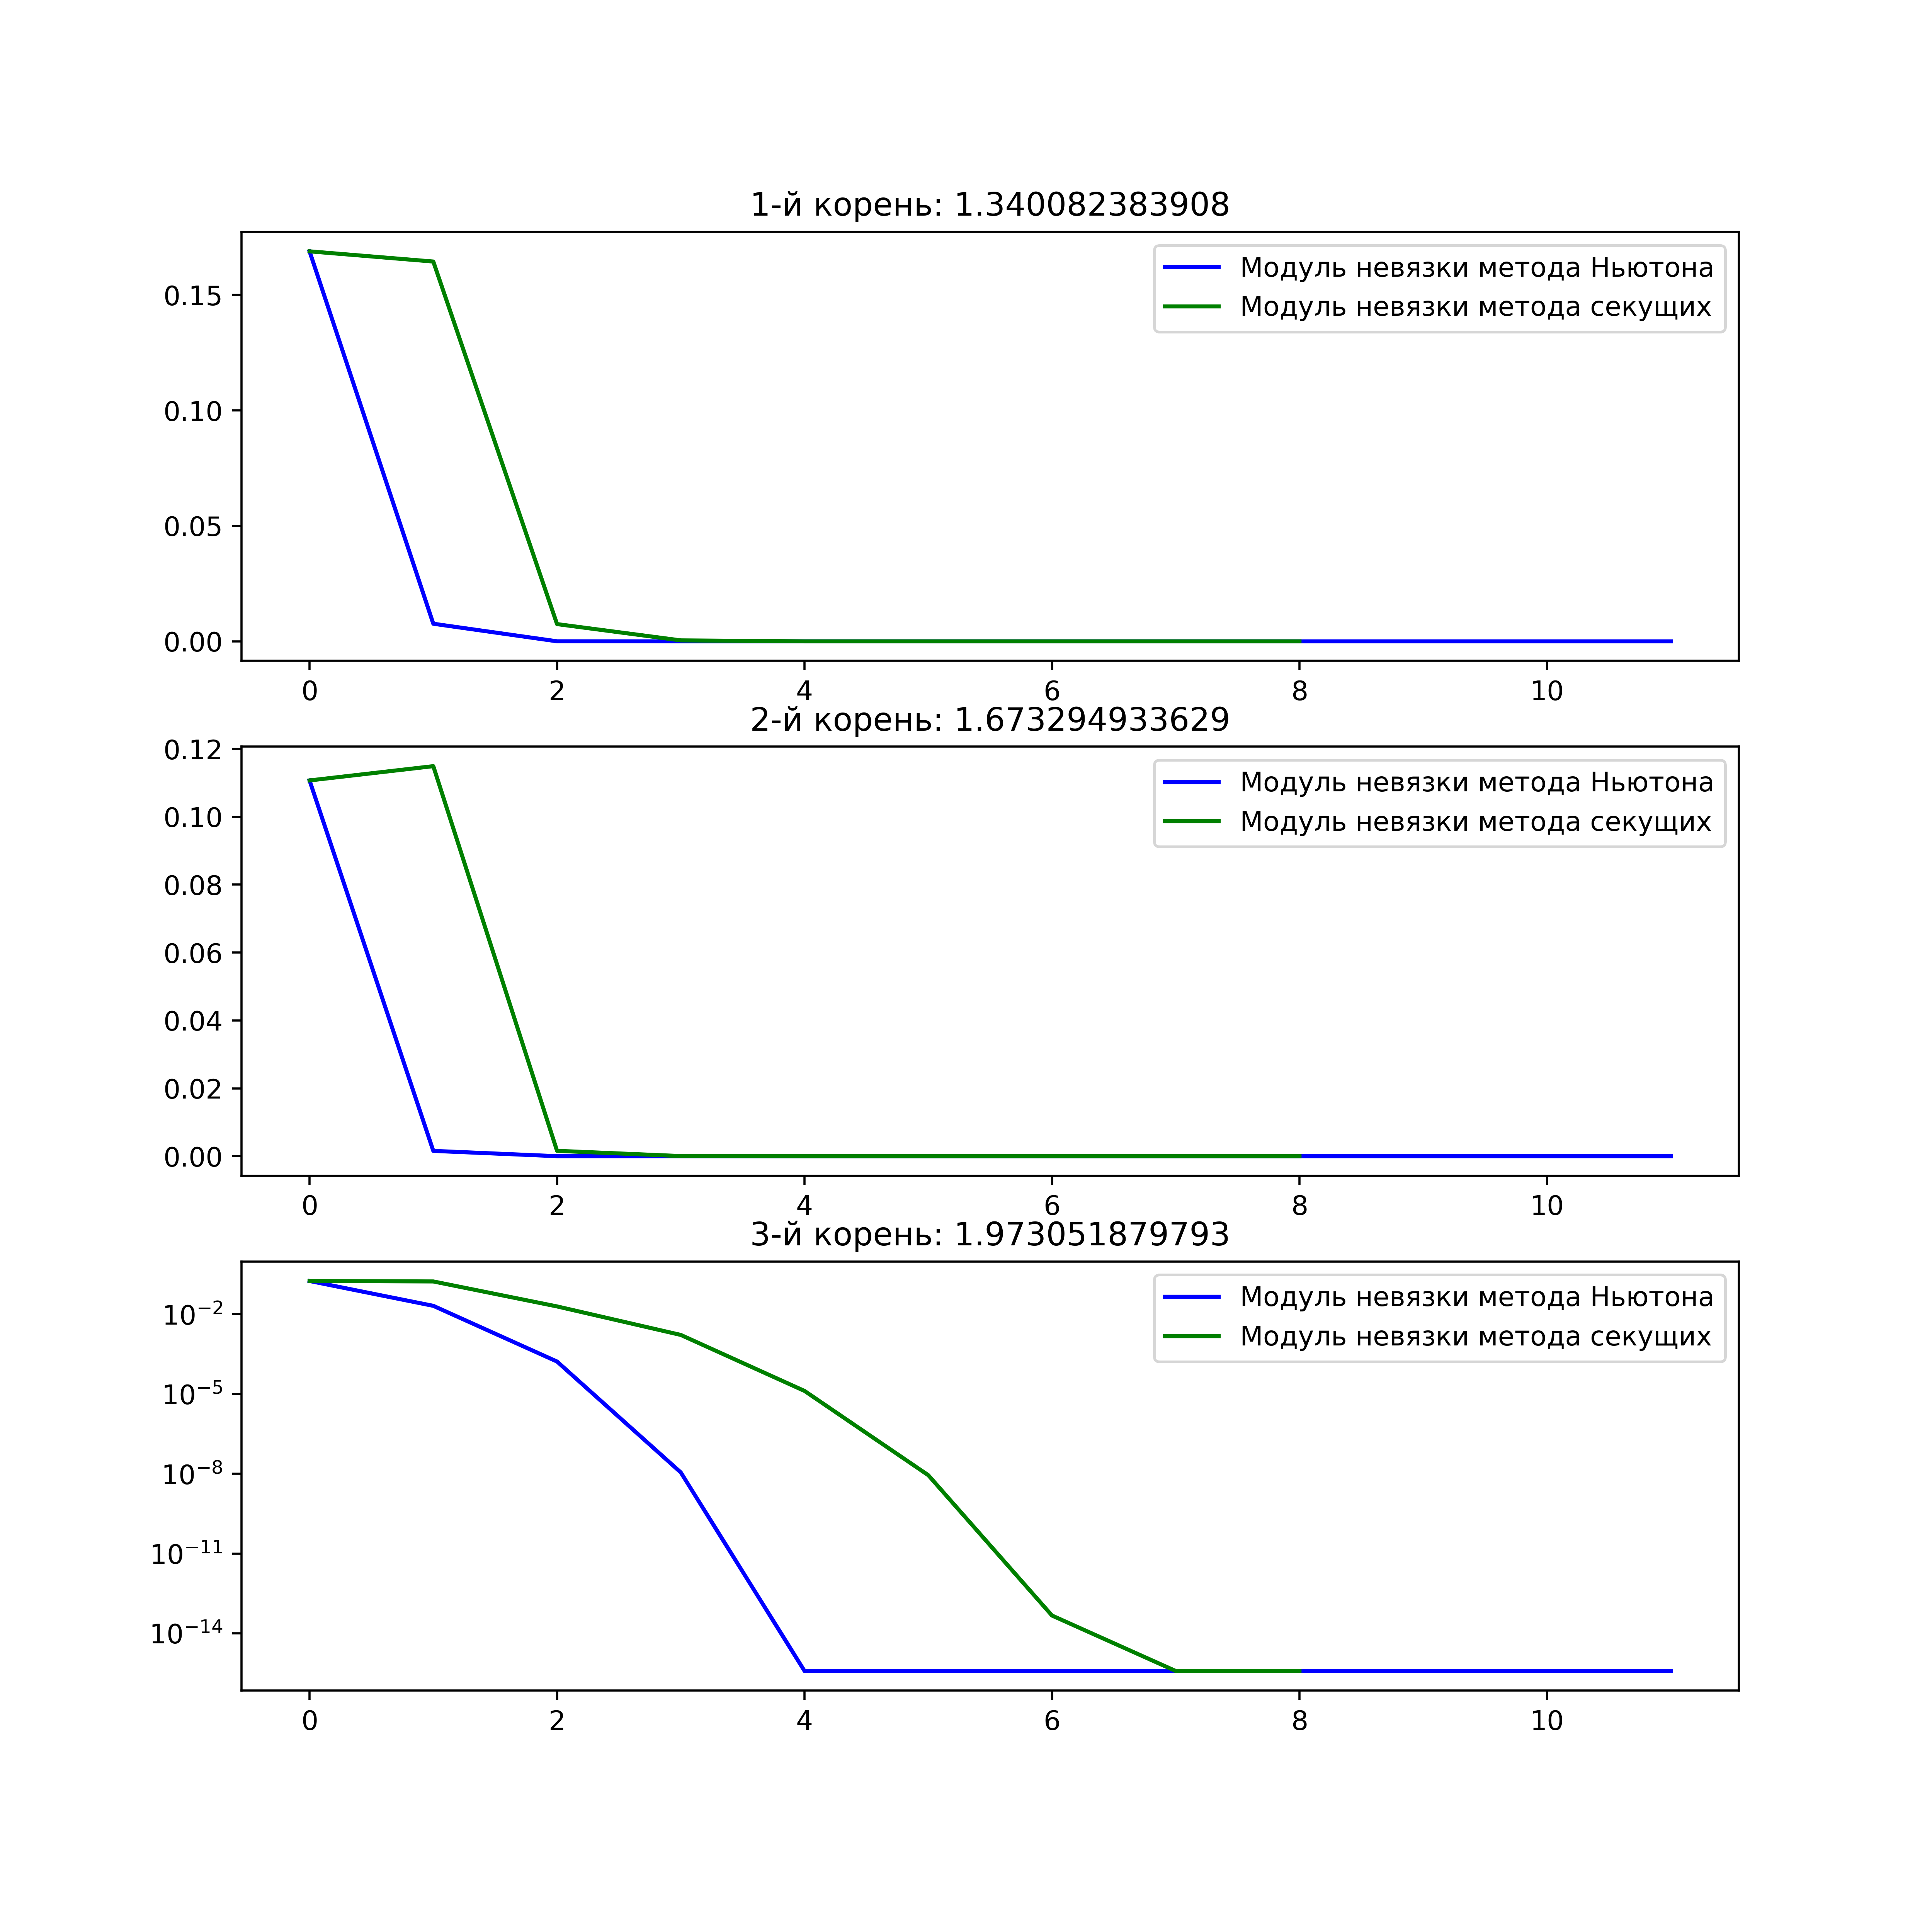
\includegraphics[height=16cm]{2.2_residual.png}

На графиках наглядно продемонстрированы различия в скорости сходимости данных методов. Метод Ньютона обладает квадратичной сходимостью ($p = 2$), в то время как порядок сходимости метода секущих составляет $p = \frac{\sqrt{5} + 1}{2} \approx 1.618$, в результате чего и получаем, что метод Ньютона "опережает" метод секущих на 1-2 итерации.

\section*{Задача 2.3}
\subsection*{Постановка задачи}
Найти корни уравнения $f(x) = 0$ и определить их кратность
\[
	f(x) = 8(\sqrt{2} - 1)\arctg{x} - \pi(\sqrt{2} - 1) - 2x(2\sqrt{2} - 1) + 7 - 4\sqrt{2} + x^2
\]
\subsection*{Решение}

Вычислим производные функции, и определим кратность корней.

\noindent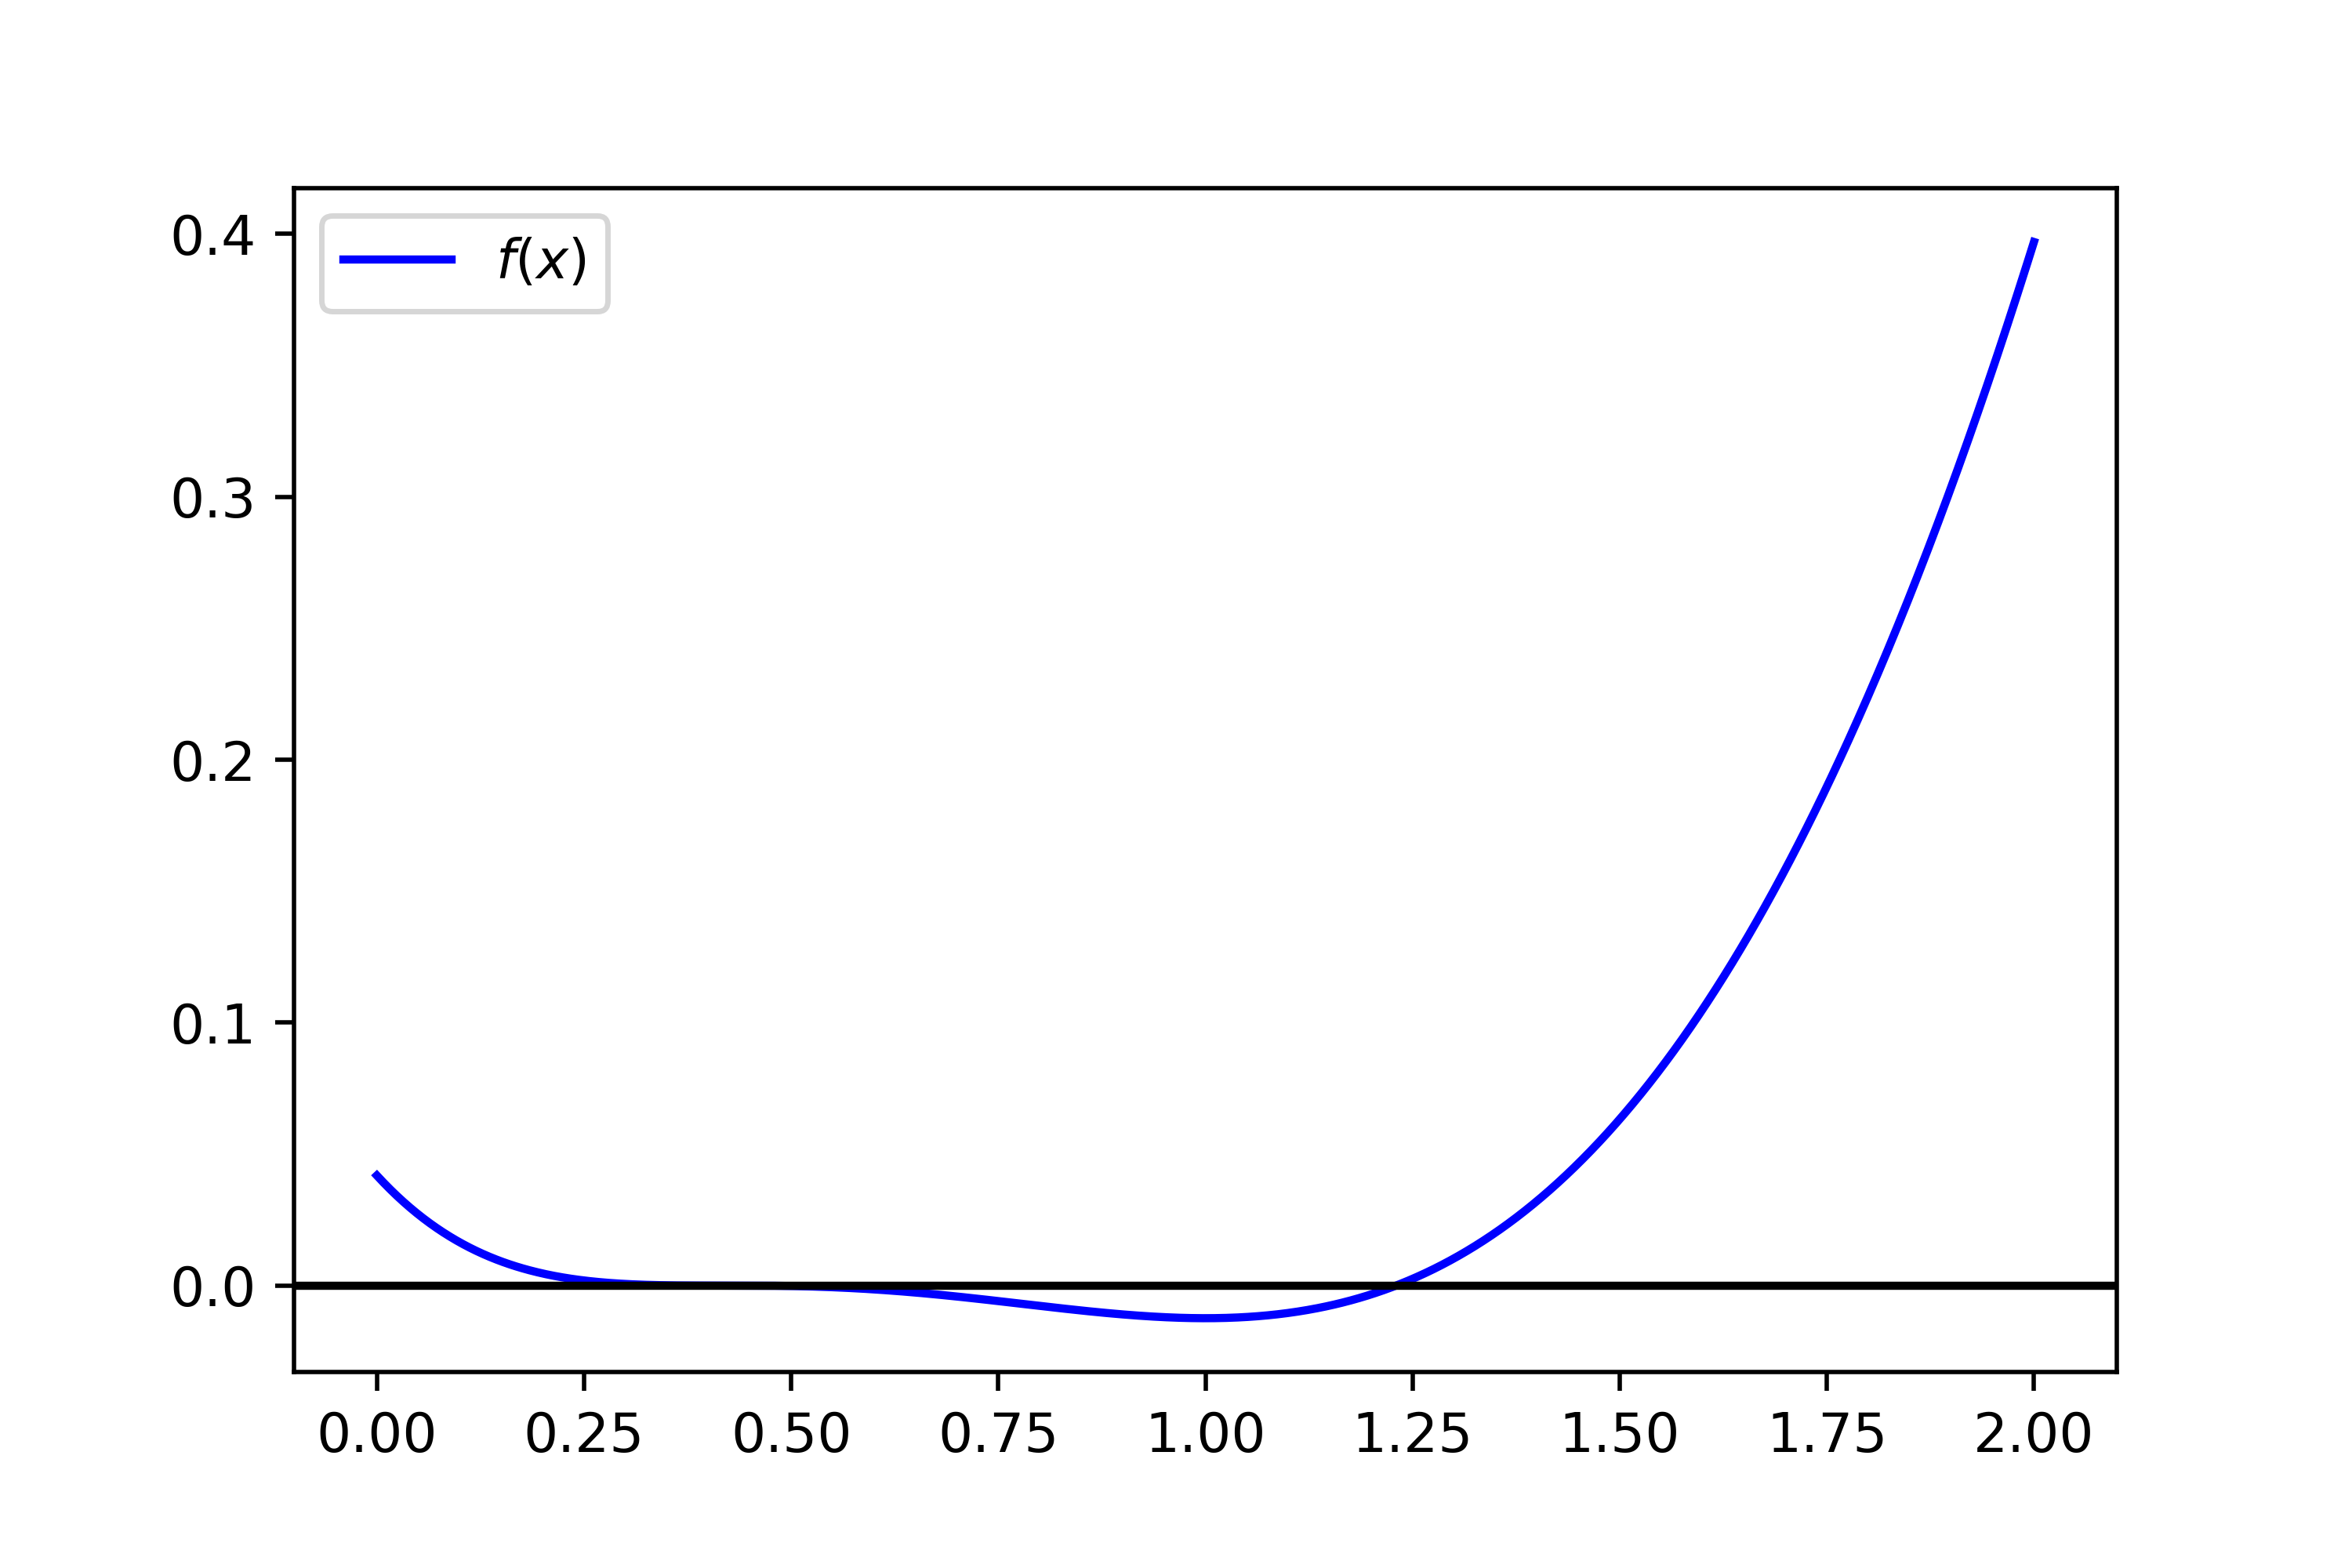
\includegraphics{2.3_plot.png}

 Получили 2 корня на следующих отрезках:

\begin{gather*}
	x_1 \in [0.4, 0.425] \\
	x_2 \in [1.2, 1.3]
\end{gather*}

Причем, как следует из графиков производных, первый корень имеет кратность 3:

\noindent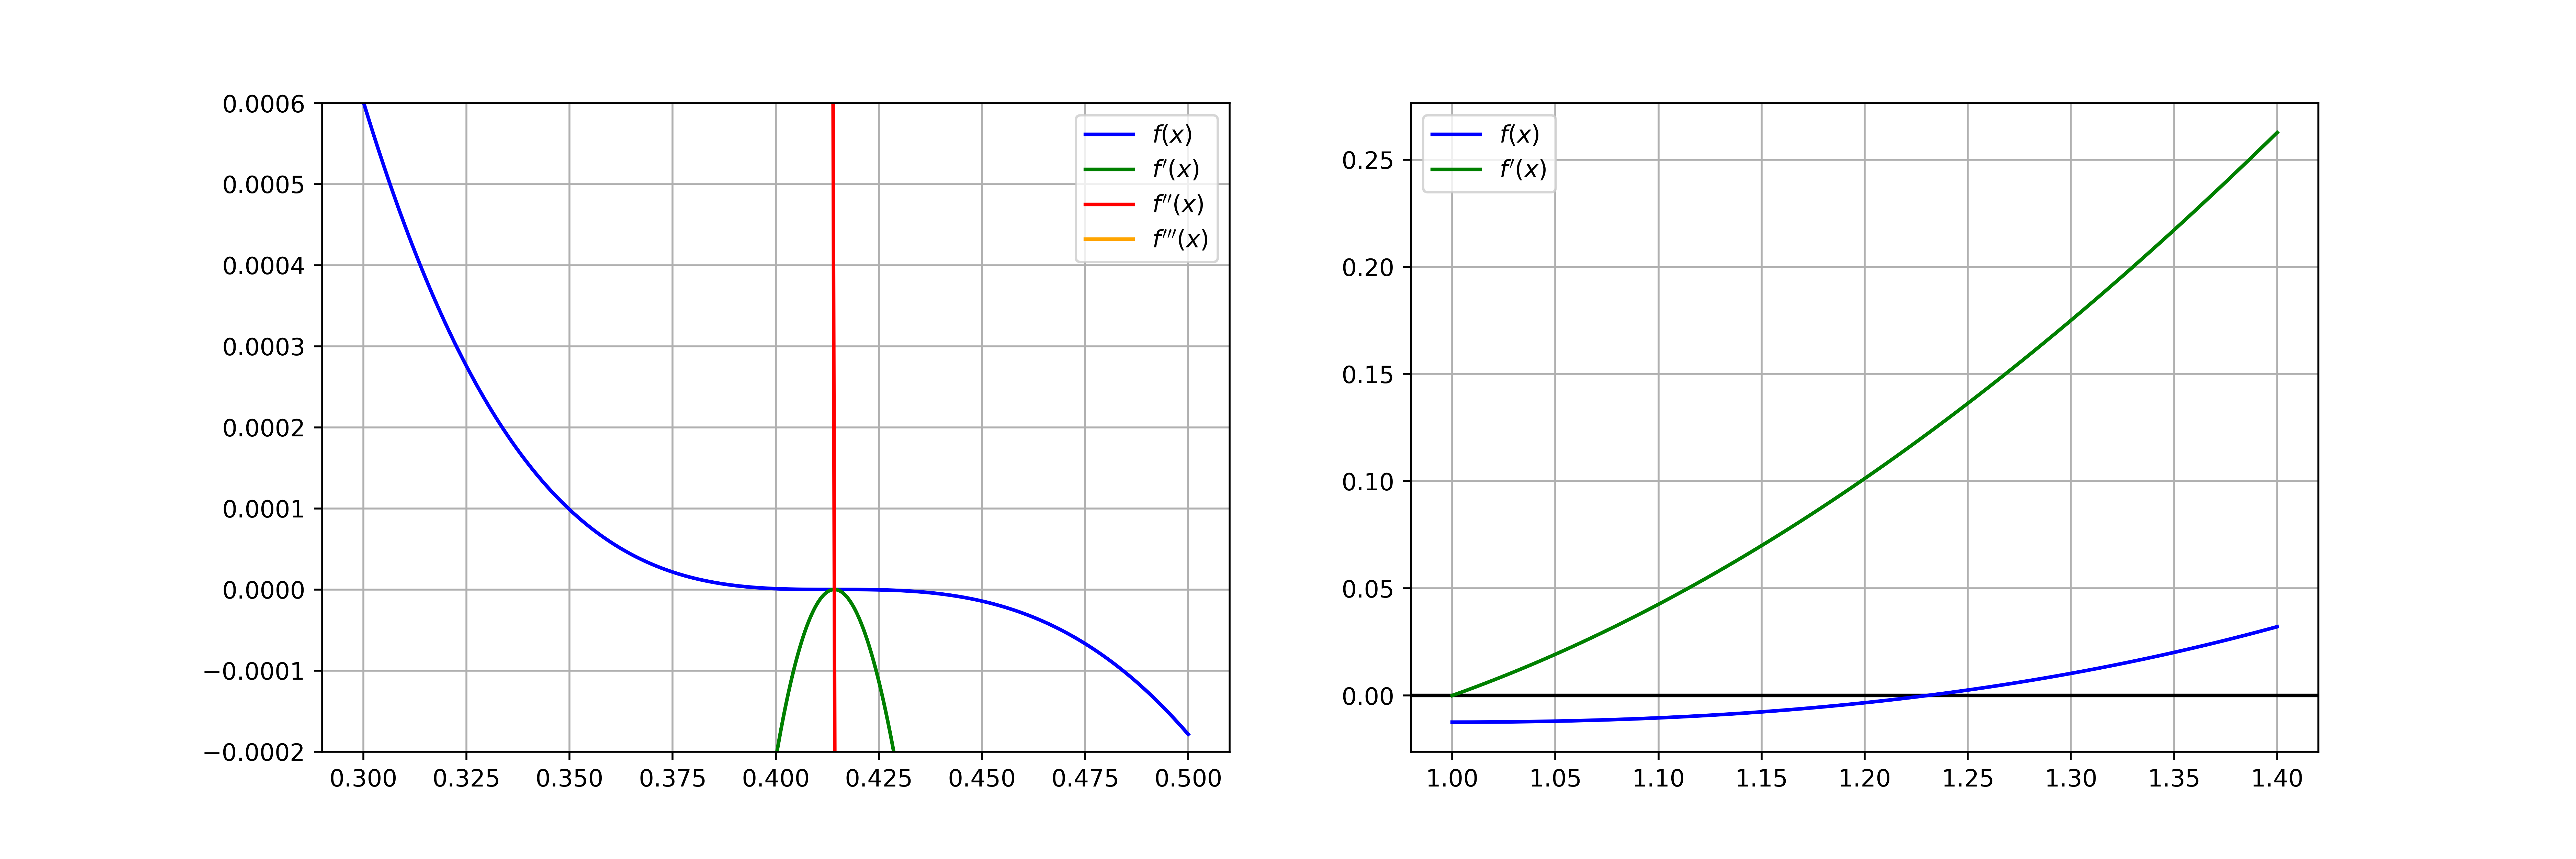
\includegraphics{2.3_plot_d.png}

Второй корень кратности 1 легко находится с помощью метода Ньютона: $ x_2 = 1.2302155532993027$

Найдем первый корень с помощью метода бисекции: $ x_1 = 0.41420254713302707 $ за 34 итерации.
Причем ни простой метод Ньютона, ни модифицированный для кратных корней не смогли приблизиться к этому значению.

Ответ: $ x_1 = 0.41420254713302707$, кратность 3; $x_2 =  1.2302155532993027$, кратность 1

\end{document}